\chapter{Implementation and Solution}
\thispagestyle{fancy}

From the three specified refactorings, \textit{Toggle Function Definition} has 
been implemented in depth. This chapter explains how the refactoring was 
implemented and which problems had to be solved during development.

\section{Implementation approach}

At the beginning, as many cases as possible were collected on the project wiki 
to gain a view on what had to be realized, what was planned to take into scope 
and what had nothing to do with toggling function definitions. Some cases were 
simple, some exotic. The simplest one, toggling from inside a class to the same 
file outside the class, was chosen to be implemented first (See listings 
\ref{funcdefPre} and \ref{funcdefPost}). 

Before, a skeleton plug-in was built with a \texttt{NullRefactoring} to try
whether it was possible to develop a separate plug-in instead of directly
manipulating the CDT source code. By this approach it was assured that the
developed plug-in may be deployed easily even without being integrated into CDT.

After the first refactoring was implemented, more cases were added by order how
a member function is toggled circularly. Mostly it was worked with a test
driven development approach. First write a test and then implement the
functionality to get a positive test restult.

\section{Architecture}

In Eclipse, most of the architecture of a plug-in is already given. Some
specialties of the toggle refactoring implementation are presented in this
section.

\subsection{Strategies}

The way to toggle from one place to another differs a lot depending on
the current position. Having all logic in the same unit would need a complex
conditional structure which is on one side confusing and on the other side
slow.

Consequently, a strategy pattern based code structure was introduced. For
toggling a simple not templated member function, three strategies were used.
With the help of these, member functions may be toggled circularly.

\begin{itemize}
\item ToggleFromClassToInHeaderStrategy
\item ToggleFromInHeaderToImplementationStrategy
\item ToggleFromImplementationHeaderOrClassStrategy
\end{itemize}

To support templated classes, another strategy is required which toggles from
\textit{in-header} back to \textit{in-class} as explained in section
\ref{templatedmember}. This strategy is specially implemented to support
templated functions.

\begin{itemize}
\item ToggleFromInHeaderToClassStrategy
\end{itemize}

All these strategies implement an interface with a \texttt{run()} method taking
a \texttt{ModificationCollector} to collect the changes to be applied to the 
source code.

\begin{lstlisting}[caption={IToggleRefactoringStrategy},
label={01templatedMember}, language=Java]
public interface IToggleRefactoringStrategy {
  public void run(ModificationCollector col);
}
\end{lstlisting}

An interface was chosen because an abstract class containing all the methods
needed by the various strategies was too big and unclear. This resulted in the
interface and a static helper class, named \texttt{ToggleNodeHelper}.

\subsection{ToggleNodeHelper}

\texttt{ToggleNodeHelper} contains a lot of methods which could be reused by
other projects. It inherits from NodeHelper to make the integration of these
methods as smooth as possible.

\subsection{Context}

The \texttt{ToggleRefactoringContext} is used to collect and store information 
about definitions, declarations and their corresponding translation units.

The context is passed then passed to the strategy factory. See \ref{factory}.
The factory passes the context to the, by itself created strategy since the
strategy is the main user of the context and retrieves all its information it.

The context was introduced to prevent the code smell \textit{Too Many 
Parameters}\cite{cwiki}. A common refactoring for this problem is to introduce a 
parameter object which consolidates all arguments.

The justification that the context searches the information by its own is due
to the fact that context would just be a very small data class and yet another
class would be needed to search and collect the information which builds and
returns the context.

\subsection{Strategy Factory}
\label{factory}

The \textit{ToggleStrategyFactory} is used to decide which strategy should be 
considered, based on the context given. The strategy makes varous checks
and decides which strategy will be returned.

\begin{lstlisting}[caption={IToggleRefactoringStrategy},
label={strategy}, language=Java]

public IToggleRefactoringStrategy getStategy() {
  if (context.getDefinition() == null) {
    throw new NotSupportedException(...
  }
  ...
  if (isInClassSituation()) {
    return new ClassToInHeaderStrategy(context);
  }
  if (isTemplateSituation()) {
    return new HeaderToClassStrategy(context);
  }
  ...
}
\end{lstlisting}

\subsection{Stopping with Exception}

%TODO: add something here

\subsection{Basic call flow}
The sequence diagram in figure \ref{sd} illustrates the basic call flow when 
\textit{Toggle Function} is invoked.
\begin{figure}[h]
  \centering
  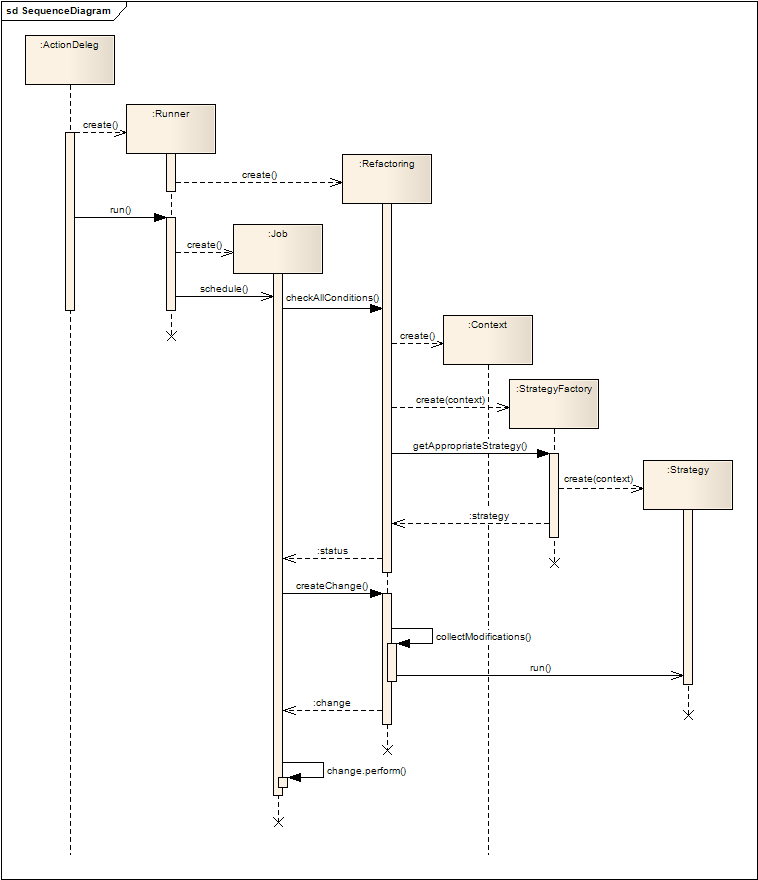
\includegraphics[width=\textwidth]{seqdiagram/SequenceDiagram.png}
  \caption{Basic call flow when toggling a function definition}
  \label{sd}
\end{figure}

\subsection{Implications of not using a refactoring wizard}
No wizard was used for this refactoring since it must be fast and may be 
executed several times in succession. When using a wizard, the 
\textit{RefactoringWizardOpenOperation} handles the execution of the refactoring 
inside a separate job. Since the toggle refactoring does not use the wizard, a 
separate job had to be scheduled by the ActionDelegate.

In addition, the undo functionality had to be implemented separately. When the 
changes are performed, they (surprisingly) also return the undo changes that are 
needed by the UndoManager. The functionality of the 
\texttt{ToggleRefactoringRunner} is described in the following section.

\subsection{Running the refactoring}\label{runnersec}
The \texttt{ToggleRefactoringRunner} is instantiated and run by the 
\texttt{Tog- glingActionDelegate}. It is responsible for running the refactoring 
in a separate job and for allowing only one toggling refactoring instance being
active. The job that is scheduled belongs to the family
\texttt{FAMILY\_TOGGLE\_DEFINITION}. This is needed to check weather there is
only one instance.

Listing \ref{runner} shows the simplified process without error checking. The 
changes are collected, executed and registered at the undo manager.

\begin{lstlisting}[caption={running the refactoring},label={runner},language=java]
status = refactoring.checkAllConditions(monitor);
change = refactoring.createChange(monitor);
change.initializeValidationData(monitor);

IUndoManager undoManager = 
    RefactoringCore.getUndoManager();
undoManager.aboutToPerformChange(change);
undoChange = change.perform(monitor);

undoChange.initializeValidationData(monitor);
undoManager.changePerformed(change, success);
undoManager.addUndo("toggling", undoChange);
\end{lstlisting}

\section{Testing and Performance Environment}

This section introduces strategies to simplify testing and monitoring of 
performance.

\subsection{Normal Testing}

The toggle refactiong plug-in was covered with tests with over 80\%. Mainly the
refactoring tests from CDT were used for default testing. The test files were
divided into the various C++ features for some simple default cases or need
special handling. These files have the inner structure in which the toggle order
was created. Namely from \textit{in-class} to \textit{in-header} to
\textit{in-implementation}.

After a problem was found, an issue was created and a test case was introduced
to the file of the specific C++ feature where the problem occurred. 

\subsection{Testing for exceptions}

Error testing is not actually an issue but the mechanism to test for exceptions 
is not obvious, so an example will be shown at this point. 

The .rts test file may include the following syntax:

\begin{lstlisting}[caption={Syntax to set variables inside a .rts file},
language=java]
//@.config
fatalerror=true
\end{lstlisting}

The \textit{fatalerror} variable may be retrieved using a member function of \textit{RefactoringTest}:
\begin{lstlisting}[caption={Accessing a property set in the .rts file},
language=java]
@Override
protected void configureRefactoring(
    Properties refactoringProperties) {
  fatalError = Boolean.valueOf(
      refactoringProperties.getProperty(
      "fatalerror", "false")).booleanValue();
}
\end{lstlisting}

The \textit{runTest} method may then assert that an error has occurred by using:
\begin{lstlisting}[caption={Checking for errors inside the refactoring test class},language=java]
RefactoringStatus initialConditions = 
    refactoring.checkInitialConditions(
    NULL_PROGRESS_MONITOR);
if (fatalError)
  assertConditionsFatalError(initialConditions);
\end{lstlisting}

All in all, the special refactoring test environment developed by \cite{GB06} 
was a big help for relaxed refactoring.

\subsection{Testing New File Creation}

In case a member function is toggled from \textit{in-header} to
\textit{in-implementation} and the implementation file does not exist, the user
of the plug-in is asked through the \texttt{ToggleFileCreator} if he wants to
create a new file and move the function there.

Long time it was not tested for this case and more than once this functionality
was hurt and destroyed by simply not testing for it. 

In the .rts file to test the toggling the \texttt{newfiles} variable has been
introduced. This variable takes one or more file names separated by a comma.

\begin{lstlisting}[caption={Syntax to set variables inside a .rts file},
language=java]
//@.config
filename=A.h
newfiles=A.cpp, B.h, C.h
//@A.h
\end{lstlisting}

Further there is no need to write the initial code state of the file since it
does not exist. However the final state must be written for comparison like
any other test.

\begin{lstlisting}[caption={Writing newfile test}]
//!FreefunctionFromHeaderToImpl
//#ch.hsr.ecl[...].ToggleRefactoringTest
//@.config
filename=A.h
newfiles=A.cpp
//@A.h
void /*$*/freefunction/*$$*/() {
    return;
}
//=
void freefunction();

//@A.cpp
//=


#include "A.h"

void freefunction()
{
    return;
}
\end{lstlisting}

The files listed in the \texttt{newfiles} variable are deleted before the
actual refactoring in the test is started. Then the new file gets created and
is compared with the expected source.

%TODO: add some words about the answer no!

\subsubsection{User Inputs}

The easiest solution to test user inputs, beeing aware that it is not the
nicest, is to Mock the Refactoring the return a internal reference to the
\texttt{ToggleRefactoringContext}. The context however has the ability to set
predefined answer values to the question of the file creation, which is done in
the test class.

\subsection{Real World Test Environment}

The toggle refactoring was tested with some open Source projects found out in
the wild.

\subsubsection{COAST}
The COAST~\cite{COAST} source code was used as test environment for real-world 
tests as it uses a lot of C++ code features to test the toggling.

Toggling some functions in COAST, we discovered that macros are not toggled
correctly and are replaced by an \texttt{NullStatement} resulting in a function
with a lot of semicolons.

\subsubsection{WebKit}
Testing to toggle functions from Webkit~\cite{Webkit} code showed us two
problems.

First Webkit uses a lot of namespaces. Until this point the Toggle
plug-in did not work correctly. Functions were moved completely out of the
namespace and were referenced with the full qualified namespace as shown in
listing \ref{wrongnamespace1}. This is not very elegant.

\begin{lstlisting}[caption={\texttt{function()} with reference to fully
qualified namespace}, label={wrongnamespace1}, language=C++]
#ifndef A_H_
#define A_H_

namespace N
class A {
  void function();
};
}

inline void N::A::function() {
  return;
}

#endif /* A_H_ */
\end{lstlisting}

The behavior was changed later to the following.

\begin{lstlisting}[caption={A.h, function definition in namespace},
label={wrongnamespace2}, language=C++]
#ifndef A_H_
#define A_H_

namespace N {
class A {
  void function();
};

inline void A::function() {
  return;
}

}

#endif /* A_H_ */
\end{lstlisting}

An other Problem discovered with Webkit was that Preprocessor Statments were
deleted. Have a look at section \ref{preprocessor} for this problem.

\subsection{Performance tests}

The simplest way to assess the speed of the refactoring is to look at the JUnit
time measurements. The first test that is run takes more time and represents the 
time needed for first time toggling when the refactoring infrastructure has to 
be loaded. 

All performance tests have been executed on the same developer machine, taking
the average time of three consecutive runs of all tests. Five scenarios have
been chosen to be able to observe the performance of the toggle refactoring:

\begin{enumerate}
\item First time toggling: Includes loading of the infrastructure and will take 
some more time.
\item Toggle from in class to header: Only one file is affected by this 
refactoring. This represents the least complex refactoring and should be the 
quickest one beside the reference test.
\item Toggle from implementation to header: Two files are affected here.
\item Emtpy reference test: A dummy refactoring that won't load and analyze any 
code. Shows what amount of time is consumed by the given refactoring 
infrastructure.
\end{enumerate}

Another technique to measure time more accurately was checked out. For this, the 
\textit{org.eclipse.test.performance} plug-in was used.
